\documentclass[10pt]{article}
\usepackage{tikz}
\usetikzlibrary{shapes.misc}
\usepackage[margin=0cm]{geometry}
\pagestyle{empty}
\tikzstyle{every node}=[cross out, draw, red]

\begin{document}

\vspace*{\fill}
\begin{center}
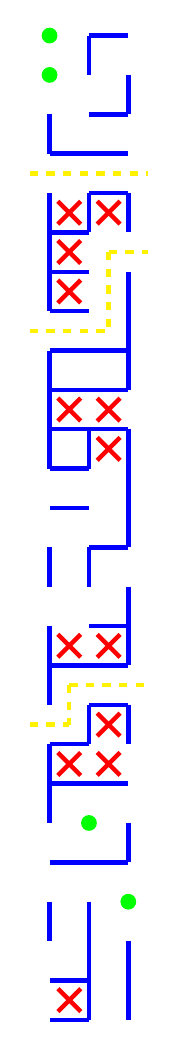
\begin{tikzpicture}[x=0.5cm, y=-0.5cm, ultra thick, blue]
% Walls
    \draw (1,0) -- (2,0);
    \draw (1,2) -- (2,2);
    \draw (0,3) -- (2,3);
    \draw (1,4) -- (2,4);
    \draw (0,5) -- (1,5);
    \draw (0,6) -- (1,6);
    \draw (0,7) -- (1,7);
    \draw (0,8) -- (2,8);
    \draw (0,9) -- (2,9);
    \draw (0,10) -- (2,10);
    \draw (0,11) -- (1,11);
    \draw (0,12) -- (1,12);
    \draw (1,13) -- (2,13);
    \draw (1,15) -- (2,15);
    \draw (0,16) -- (2,16);
    \draw (1,17) -- (2,17);
    \draw (0,18) -- (1,18);
    \draw (0,19) -- (2,19);
    \draw (0,21) -- (2,21);
    \draw (0,24) -- (1,24);
    \draw (0,25) -- (1,25);
    \draw (0,2) -- (0,3);
    \draw (0,4) -- (0,7);
    \draw (0,8) -- (0,11);
    \draw (0,13) -- (0,14);
    \draw (0,15) -- (0,17);
    \draw (0,18) -- (0,20);
    \draw (0,22) -- (0,23);
    \draw (1,0) -- (1,1);
    \draw (1,4) -- (1,5);
    \draw (1,10) -- (1,11);
    \draw (1,13) -- (1,14);
    \draw (1,17) -- (1,18);
    \draw (1,22) -- (1,25);
    \draw (2,1) -- (2,2);
    \draw (2,4) -- (2,5);
    \draw (2,6) -- (2,9);
    \draw (2,10) -- (2,13);
    \draw (2,14) -- (2,16);
    \draw (2,17) -- (2,18);
    \draw (2,20) -- (2,21);
    \draw (2,23) -- (2,25);
% Pillars
    \fill[green] (0,0) circle(0.2);
    \fill[green] (0,1) circle(0.2);
    \fill[green] (1,20) circle(0.2);
    \fill[green] (2,22) circle(0.2);
% Inner points in accessible cul-de-sacs
    \node at (0.5,4.5) {};
    \node at (1.5,4.5) {};
    \node at (0.5,5.5) {};
    \node at (0.5,6.5) {};
    \node at (0.5,9.5) {};
    \node at (1.5,9.5) {};
    \node at (1.5,10.5) {};
    \node at (0.5,15.5) {};
    \node at (1.5,15.5) {};
    \node at (1.5,17.5) {};
    \node at (0.5,18.5) {};
    \node at (1.5,18.5) {};
    \node at (0.5,24.5) {};
% Entry-exit paths without intersections
    \draw[dashed, yellow] (-0.5,3.5) -- (2.5,3.5);
    \draw[dashed, yellow] (1.5,5.5) -- (2.5,5.5);
    \draw[dashed, yellow] (-0.5,7.5) -- (1.5,7.5);
    \draw[dashed, yellow] (0.5,16.5) -- (2.5,16.5);
    \draw[dashed, yellow] (-0.5,17.5) -- (0.5,17.5);
    \draw[dashed, yellow] (0.5,16.5) -- (0.5,17.5);
    \draw[dashed, yellow] (1.5,5.5) -- (1.5,7.5);
\end{tikzpicture}
\end{center}
\vspace*{\fill}

\end{document}
